\begin{framed}

Objetivos:
\begin{itemize}
    \item Modelar el efecto de la viscosidad en flujos cercanos a una pared.
    \item Mostrar las distintas definiciones de capa límite.
\end{itemize}

Contenidos:
\begin{itemize}
    \item Flujo viscoso sobre una placa plana.
    \item La capa límite y su espesor.
    \item El espesor de desplazamiento.
    \item El espesor de momentum.
\end{itemize}

Bibliografía:
\begin{itemize}
    \item White, F. M. (2008) Mecánica de Fluidos. McGraw-Hill. Sexta edición. Secciones 4.1-4.4
    \item Fox, R. W., Pritchard, P. J. y McDonald, A. T. (2009) Introduction to Fluid Mechanics. John Wiley \& Sons. Secciones 7.1-7.3
\end{itemize}
\end{framed}

\section*{Flujo viscoso sobre una superficie}

Hace algunas clases estuvimos estudiando flujo potencial, el cual era no viscoso.
Una implicancia de su ``no viscosidad'' era que la condición de borde en una pared era de impermeabilidad ($\mathbf{V}\cdot\mathbf{n}=0$), sin embargo, el flujo podía deslizarse.
Obviamente, sabemos que no existe tal cosa como un flujo ``no viscoso''. 
De hecho, experimentalmente podemos ver que la velocidad del fluido en la interfaz con el sólido es igual a la velocidad del sólido, en otras palabras, el fluido no desliza.
%
\begin{figure}[!h]
\centering
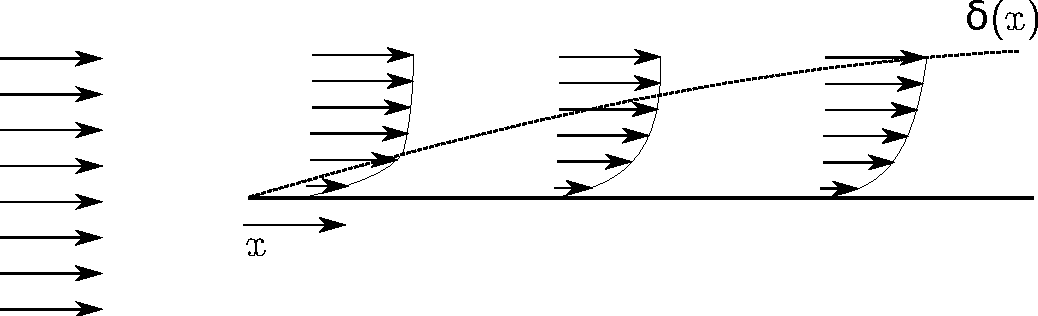
\includegraphics[width=0.8\textwidth]{clase08/capa_limite.pdf}
\caption{Flujo sobre una placa plana.}
\label{fig:capa_limite}
\end{figure}
%
Tomemos, por ejemplo, el flujo uniforme que se topa con una placa plana en la Figura \ref{fig:capa_limite}.
Lo que esperamos que ocurra es que el flujo en la placa tenga velocidad cero, y de ahí vaya creciendo paulatinamente hasta llegar a la velocidad de entrada $U_\infty$.
En el principio de la placa (a $x$ pequeño), esperaríamos que el efecto de la placa no llega muy lejos, y la velocidad rápidamente retoma $U_\infty$, sin embargo, aguas abajo, el efecto de la placa llega mucho más adentro en el flujo, y este efecto crece a medida que nos movemos a lo largo de ella.
Esta zona de influencia de la placa se conoce como \emph{capa límite}, y su espesor se representa como $\delta$.
En la FIgura \ref{fig:capa_limite}, la capa límite está representada por la línea punteada.
El flujo fuera de la capa límite es un flujo uniforme que perfectamente puede ser modelado como un flujo uniforme potencial, a pesar que sepamos que el fluido tiene viscosidad, pero afuera de la capa límite el efecto de la viscosidad es despreciable.

\section*{Definiciones de capa límite}
Una pregunta válida es \mbox{?`}dónde consideramos que el flujo finalmente a retomado su velocidad $U_\infty$? 
En otras palabras, \mbox{?`}cuál es el criterio para dibujar la línea punteada en la Figura \ref{fig:capa_limite}?
Aquí simplemente tenemos que ponernos de acuerdo, y la convención dice que consideraremos que el fin de la capa límite se encuentra donde la velocidad paralela a la placa ha alcanzado $0.99U_\infty$.
